\chapter{Síntesis de Sonidos mediante Modelos Físicos}

\section{Introducción}
Se utilizó el modelo de Karplus-Strong para sintetizar el sonido de instrumentos de cuerda percutida u otros tipos de percusión. Este algoritmo, creado por Kevin Karplus y Alexander Strong en 1983 para sintetizar sonidos con pocos recursos y a tiempo real.

En este trabajo se analizaron el modelo básico para la síntesis de cuerdas percutidas y el modelo modificado para la síntesis de instrumentos de percusión.

\section{Modelo Conceptual}

En principio se trata de un sistema linear excitado con una secuencia aleatoria de longitud finita. Consiste de una línea de retarde de L muestras retroalimentadas mediante un filtro.

\begin{figure}[ht]
    \centering
    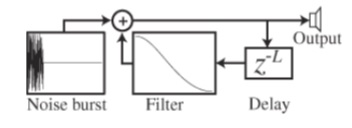
\includegraphics{res/ks_concept.jpg}
    \caption{Diagrama Conceptual del Modelo de Karplus-Strong}
    \label{fig:KS_model}
\end{figure}


Los parámetros disponibles para su control son tono, amplitud y tiempo de decaimiento.

El tono es espicificado por un entero aproximadamente igual al período del sonido, en muestras.
La amplitud es especificada por el pico inicial de amplitud A.
El tiempo de decaimiento es determinado por el tono y el factor de estiramiento de decaimiento	S.